\qs{}{
    How many students are enrolled per subject?
}

Retrieve the number of students enrolled in each subject by joining the \texttt{course} and \texttt{enrollment} tables based on the course ID. \texttt{GROUP} the results by course name and \texttt{COUNT} the distinct student IDs to determine how many students are enrolled in each subject. The results are sorted in descending order using \texttt{DESC} to show the subjects with the highest enrollment first.
\vspace{\baselineskip}

\sol{}
\noindent\line(1, 0){0.89\linewidth}
\begin{verbatim}
SELECT c.crs_name AS Subject, COUNT(DISTINCT e.stud_id) AS Number_of_Students
FROM course c
LEFT JOIN enrollment e ON c.crs_id = e.crs_id
GROUP BY c.crs_name
ORDER BY Number_of_Students DESC;
\end{verbatim}
\noindent\line(1, 0){\linewidth}

\begin{figure}[H]
    \centering
    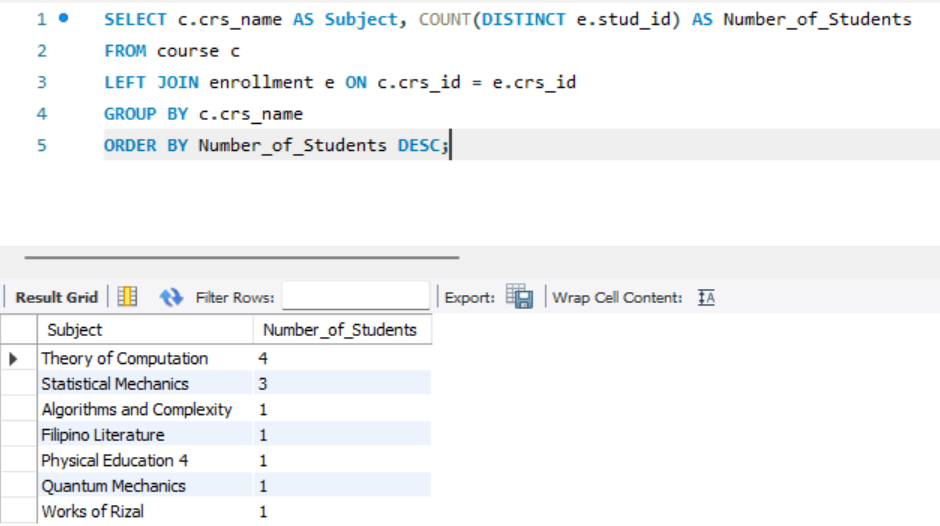
\includegraphics[width=0.7\linewidth]{images/q3.png}
    \caption{Question 3 Query and Output}
\end{figure}
